
\begin{figure}
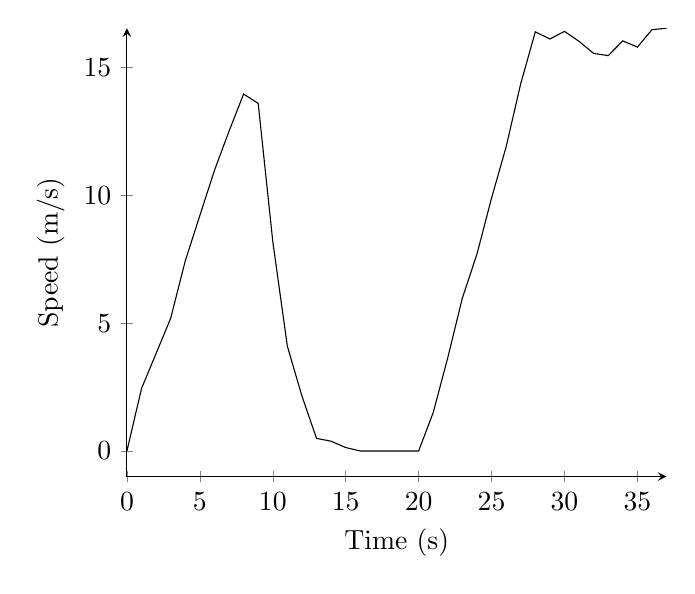
\begin{tikzpicture}
\begin{axis}[
legend style={anchor=west},
axis x line=bottom,
axis y line=left,
ymin=-1,
xlabel=Time (s),
ylabel=Speed (m/s),
]
\addplot[] coordinates {
(0, 0.0)
(1, 2.44255984318)
(2, 3.81596629217)
(3, 5.1931042067)
(4, 7.43826163147)
(5, 9.21204036189)
(6, 10.9777619914)
(7, 12.5129254552)
(8, 13.9663839334)
(9, 13.6018793792)
(10, 8.19888697661)
(11, 4.09776660895)
(12, 2.14793310363)
(13, 0.493644308871)
(14, 0.383089654847)
(15, 0.134744394734)
(16, 0.0)
(17, 0.0)
(18, 0.0)
(19, 0.0)
(20, 0.0)
(21, 1.50412517251)
(22, 3.65321244841)
(23, 5.9876129881)
(24, 7.70625115954)
(25, 9.8962233754)
(26, 11.902530677)
(27, 14.3717962518)
(28, 16.400728806)
(29, 16.1210633599)
(30, 16.4189737165)
(31, 16.0283511894)
(32, 15.5556866157)
(33, 15.4711267919)
(34, 16.0479740213)
(35, 15.8024057006)
(36, 16.4862493)
(37, 16.5424294432)
};

\end{axis}
\end{tikzpicture}
\label{tik:0:2}
\caption{0 percent diving with GSC on route $2$}
\end{figure}
